\documentclass[twoside]{book}

% Packages required by doxygen
\usepackage{fixltx2e}
\usepackage{calc}
\usepackage{doxygen}
\usepackage[export]{adjustbox} % also loads graphicx
\usepackage{graphicx}
\usepackage[utf8]{inputenc}
\usepackage{makeidx}
\usepackage{multicol}
\usepackage{multirow}
\PassOptionsToPackage{warn}{textcomp}
\usepackage{textcomp}
\usepackage[nointegrals]{wasysym}
\usepackage[table]{xcolor}

% Font selection
\usepackage[T1]{fontenc}
\usepackage[scaled=.90]{helvet}
\usepackage{courier}
\usepackage{amssymb}
\usepackage{sectsty}
\renewcommand{\familydefault}{\sfdefault}
\allsectionsfont{%
  \fontseries{bc}\selectfont%
  \color{darkgray}%
}
\renewcommand{\DoxyLabelFont}{%
  \fontseries{bc}\selectfont%
  \color{darkgray}%
}
\newcommand{\+}{\discretionary{\mbox{\scriptsize$\hookleftarrow$}}{}{}}

% Page & text layout
\usepackage{geometry}
\geometry{%
  a4paper,%
  top=2.5cm,%
  bottom=2.5cm,%
  left=2.5cm,%
  right=2.5cm%
}
\tolerance=750
\hfuzz=15pt
\hbadness=750
\setlength{\emergencystretch}{15pt}
\setlength{\parindent}{0cm}
\setlength{\parskip}{3ex plus 2ex minus 2ex}
\makeatletter
\renewcommand{\paragraph}{%
  \@startsection{paragraph}{4}{0ex}{-1.0ex}{1.0ex}{%
    \normalfont\normalsize\bfseries\SS@parafont%
  }%
}
\renewcommand{\subparagraph}{%
  \@startsection{subparagraph}{5}{0ex}{-1.0ex}{1.0ex}{%
    \normalfont\normalsize\bfseries\SS@subparafont%
  }%
}
\makeatother

% Headers & footers
\usepackage{fancyhdr}
\pagestyle{fancyplain}
\fancyhead[LE]{\fancyplain{}{\bfseries\thepage}}
\fancyhead[CE]{\fancyplain{}{}}
\fancyhead[RE]{\fancyplain{}{\bfseries\leftmark}}
\fancyhead[LO]{\fancyplain{}{\bfseries\rightmark}}
\fancyhead[CO]{\fancyplain{}{}}
\fancyhead[RO]{\fancyplain{}{\bfseries\thepage}}
\fancyfoot[LE]{\fancyplain{}{}}
\fancyfoot[CE]{\fancyplain{}{}}
\fancyfoot[RE]{\fancyplain{}{\bfseries\scriptsize 制作者 Doxygen }}
\fancyfoot[LO]{\fancyplain{}{\bfseries\scriptsize 制作者 Doxygen }}
\fancyfoot[CO]{\fancyplain{}{}}
\fancyfoot[RO]{\fancyplain{}{}}
\renewcommand{\footrulewidth}{0.4pt}
\renewcommand{\chaptermark}[1]{%
  \markboth{#1}{}%
}
\renewcommand{\sectionmark}[1]{%
  \markright{\thesection\ #1}%
}

% Indices & bibliography
\usepackage{natbib}
\usepackage[titles]{tocloft}
\setcounter{tocdepth}{3}
\setcounter{secnumdepth}{5}
\makeindex

% Hyperlinks (required, but should be loaded last)
\usepackage{ifpdf}
\ifpdf
  \usepackage[pdftex,pagebackref=true]{hyperref}
\else
  \usepackage[ps2pdf,pagebackref=true]{hyperref}
\fi
\hypersetup{%
  colorlinks=true,%
  linkcolor=blue,%
  citecolor=blue,%
  unicode%
}

% Custom commands
\newcommand{\clearemptydoublepage}{%
  \newpage{\pagestyle{empty}\cleardoublepage}%
}

\usepackage{caption}
\captionsetup{labelsep=space,justification=centering,font={bf},singlelinecheck=off,skip=4pt,position=top}

%===== C O N T E N T S =====

\begin{document}

% Titlepage & ToC
\hypersetup{pageanchor=false,
             bookmarksnumbered=true,
             pdfencoding=unicode
            }
\pagenumbering{roman}
\begin{titlepage}
\vspace*{7cm}
\begin{center}%
{\Large C++ Lab \\[1ex]\large 1.\+0.\+0 }\\
\vspace*{1cm}
{\large 制作者 Doxygen 1.8.11}\\
\end{center}
\end{titlepage}
\clearemptydoublepage
\tableofcontents
\clearemptydoublepage
\pagenumbering{arabic}
\hypersetup{pageanchor=true}

%--- Begin generated contents ---
\chapter{继承关系索引}
\section{类继承关系}
此继承关系列表按字典顺序粗略的排序\+: \begin{DoxyCompactList}
\item \contentsline{section}{O\+O\+S\+TK}{\pageref{classOOSTK}}{}
\item \contentsline{section}{P\+O\+S\+TK}{\pageref{structPOSTK}}{}
\item \contentsline{section}{Q\+U\+E2S}{\pageref{classQUE2S}}{}
\item \contentsline{section}{S\+T\+A\+CK}{\pageref{classSTACK}}{}
\begin{DoxyCompactList}
\item \contentsline{section}{Q\+U\+E\+IS}{\pageref{classQUEIS}}{}
\end{DoxyCompactList}
\end{DoxyCompactList}

\chapter{类索引}
\section{类列表}
这里列出了所有类、结构、联合以及接口定义等,并附带简要说明\+:\begin{DoxyCompactList}
\item\contentsline{section}{\hyperlink{classOOSTK}{O\+O\+S\+TK} }{\pageref{classOOSTK}}{}
\item\contentsline{section}{\hyperlink{structPOSTK}{P\+O\+S\+TK} }{\pageref{structPOSTK}}{}
\item\contentsline{section}{\hyperlink{classQUE2S}{Q\+U\+E2S} }{\pageref{classQUE2S}}{}
\item\contentsline{section}{\hyperlink{classQUEIS}{Q\+U\+E\+IS} }{\pageref{classQUEIS}}{}
\item\contentsline{section}{\hyperlink{classSTACK}{S\+T\+A\+CK} }{\pageref{classSTACK}}{}
\end{DoxyCompactList}

\chapter{文件索引}
\section{文件列表}
这里列出了所有文档化的文件,并附带简要说明\+:\begin{DoxyCompactList}
\item\contentsline{section}{src/\hyperlink{oostk_8h}{oostk.\+h} \\*Header file for object-\/oriented stack }{\pageref{oostk_8h}}{}
\item\contentsline{section}{src/\hyperlink{postk_8h}{postk.\+h} \\*Header file for process-\/oriented stack }{\pageref{postk_8h}}{}
\item\contentsline{section}{src/\hyperlink{que2s_8h}{que2s.\+h} \\*Header file for queue consisting of 2 stack }{\pageref{que2s_8h}}{}
\item\contentsline{section}{src/\hyperlink{queis_8h}{queis.\+h} \\*Header file for queue inheriting from stack }{\pageref{queis_8h}}{}
\item\contentsline{section}{src/\hyperlink{stack_8h}{stack.\+h} \\*Header file for operator overload object-\/oriented stack }{\pageref{stack_8h}}{}
\end{DoxyCompactList}

\chapter{类说明}
\hypertarget{classOOSTK}{}\section{O\+O\+S\+T\+K类 参考}
\label{classOOSTK}\index{O\+O\+S\+TK@{O\+O\+S\+TK}}
\subsection*{Public 成员函数}
\begin{DoxyCompactItemize}
\item 
{\bfseries O\+O\+S\+TK} (int m)\hypertarget{classOOSTK_af1012889d2e4e1ef9acfbe107feb241e}{}\label{classOOSTK_af1012889d2e4e1ef9acfbe107feb241e}

\item 
{\bfseries O\+O\+S\+TK} (const \hyperlink{classOOSTK}{O\+O\+S\+TK} \&s)\hypertarget{classOOSTK_aff2d32aaf48160e5b1ad971445ce8f15}{}\label{classOOSTK_aff2d32aaf48160e5b1ad971445ce8f15}

\item 
int {\bfseries size} (void) const \hypertarget{classOOSTK_a1c669595dd6c02f12f73c6682e7ca068}{}\label{classOOSTK_a1c669595dd6c02f12f73c6682e7ca068}

\item 
int {\bfseries how\+Many} (void) const \hypertarget{classOOSTK_a836995fe52d01742772caf5352d8b442}{}\label{classOOSTK_a836995fe52d01742772caf5352d8b442}

\item 
int {\bfseries getelem} (int x) const \hypertarget{classOOSTK_a6585038cd5bd92fd24e6ef735778195d}{}\label{classOOSTK_a6585038cd5bd92fd24e6ef735778195d}

\item 
\hyperlink{classOOSTK}{O\+O\+S\+TK} \& {\bfseries push} (int e)\hypertarget{classOOSTK_a352fdeb1209f0de9512c827cd0611117}{}\label{classOOSTK_a352fdeb1209f0de9512c827cd0611117}

\item 
\hyperlink{classOOSTK}{O\+O\+S\+TK} \& {\bfseries pop} (int \&e)\hypertarget{classOOSTK_aa0f59937c3dd01d09da5975fe7618f96}{}\label{classOOSTK_aa0f59937c3dd01d09da5975fe7618f96}

\item 
\hyperlink{classOOSTK}{O\+O\+S\+TK} \& {\bfseries assign} (const \hyperlink{classOOSTK}{O\+O\+S\+TK} \&s)\hypertarget{classOOSTK_a396ca951fcee87832141d86213cc661c}{}\label{classOOSTK_a396ca951fcee87832141d86213cc661c}

\item 
void {\bfseries print} (void) const \hypertarget{classOOSTK_a343813b38df610cb507884df82715415}{}\label{classOOSTK_a343813b38df610cb507884df82715415}

\end{DoxyCompactItemize}


\subsection{详细描述}


在文件 oostk.\+h 第 13 行定义.



该类的文档由以下文件生成\+:\begin{DoxyCompactItemize}
\item 
src/\hyperlink{oostk_8h}{oostk.\+h}\end{DoxyCompactItemize}

\hypertarget{structPOSTK}{}\section{P\+O\+S\+T\+K结构体 参考}
\label{structPOSTK}\index{P\+O\+S\+TK@{P\+O\+S\+TK}}
\subsection*{Public 属性}
\begin{DoxyCompactItemize}
\item 
int $\ast$ {\bfseries elems}\hypertarget{structPOSTK_a03fa273646d4ea4e3961694a5820e96d}{}\label{structPOSTK_a03fa273646d4ea4e3961694a5820e96d}

\item 
int {\bfseries max}\hypertarget{structPOSTK_a6ab28fe045a6fa3ad9686440ae25770f}{}\label{structPOSTK_a6ab28fe045a6fa3ad9686440ae25770f}

\item 
int {\bfseries pos}\hypertarget{structPOSTK_abdfaae2468a5aabeb5438b67cfe2bbc4}{}\label{structPOSTK_abdfaae2468a5aabeb5438b67cfe2bbc4}

\end{DoxyCompactItemize}


\subsection{详细描述}


在文件 postk.\+h 第 13 行定义.



该结构体的文档由以下文件生成\+:\begin{DoxyCompactItemize}
\item 
src/\hyperlink{postk_8h}{postk.\+h}\end{DoxyCompactItemize}

\hypertarget{classQUE2S}{}\section{Q\+U\+E2\+S类 参考}
\label{classQUE2S}\index{Q\+U\+E2S@{Q\+U\+E2S}}
\subsection*{Public 成员函数}
\begin{DoxyCompactItemize}
\item 
{\bfseries Q\+U\+E2S} (int m)\hypertarget{classQUE2S_a1c32e8ef08e7c8ea6249a6318dcae8c0}{}\label{classQUE2S_a1c32e8ef08e7c8ea6249a6318dcae8c0}

\item 
{\bfseries Q\+U\+E2S} (const \hyperlink{classQUE2S}{Q\+U\+E2S} \&q)\hypertarget{classQUE2S_aa4bdcad6821d11425491e60118fe85f1}{}\label{classQUE2S_aa4bdcad6821d11425491e60118fe85f1}

\item 
\hyperlink{classQUE2S_a8baa6f65d5fccfa902ae6f8b66ed84f5}{operator int} (void) const \hypertarget{classQUE2S_a8baa6f65d5fccfa902ae6f8b66ed84f5}{}\label{classQUE2S_a8baa6f65d5fccfa902ae6f8b66ed84f5}

\begin{DoxyCompactList}\small\item\em type casting \end{DoxyCompactList}\item 
\hyperlink{classQUE2S}{Q\+U\+E2S} \& {\bfseries operator$<$$<$} (int e)\hypertarget{classQUE2S_a49358209d2bcc7f85e74b6323c49e983}{}\label{classQUE2S_a49358209d2bcc7f85e74b6323c49e983}

\item 
\hyperlink{classQUE2S}{Q\+U\+E2S} \& {\bfseries operator$>$$>$} (int \&e)\hypertarget{classQUE2S_a8a7bc53ccf3e2cdd5416caff5feb5d22}{}\label{classQUE2S_a8a7bc53ccf3e2cdd5416caff5feb5d22}

\item 
\hyperlink{classQUE2S}{Q\+U\+E2S} \& {\bfseries operator=} (const \hyperlink{classQUE2S}{Q\+U\+E2S} \&q)\hypertarget{classQUE2S_abd2b18e0cc36cccf4110f129e9e4f8ed}{}\label{classQUE2S_abd2b18e0cc36cccf4110f129e9e4f8ed}

\item 
void {\bfseries print} (void) const \hypertarget{classQUE2S_ae1fa70c73674f87610db5f7c29dc671e}{}\label{classQUE2S_ae1fa70c73674f87610db5f7c29dc671e}

\end{DoxyCompactItemize}


\subsection{详细描述}


在文件 que2s.\+h 第 13 行定义.



该类的文档由以下文件生成\+:\begin{DoxyCompactItemize}
\item 
src/\hyperlink{que2s_8h}{que2s.\+h}\end{DoxyCompactItemize}

\hypertarget{classQUEIS}{}\section{Q\+U\+E\+I\+S类 参考}
\label{classQUEIS}\index{Q\+U\+E\+IS@{Q\+U\+E\+IS}}


类 Q\+U\+E\+IS 继承关系图\+:
\nopagebreak
\begin{figure}[H]
\begin{center}
\leavevmode
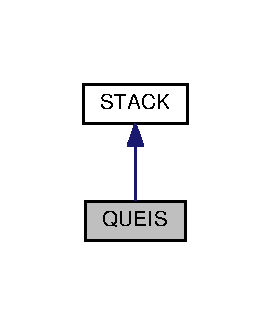
\includegraphics[width=130pt]{classQUEIS__inherit__graph}
\end{center}
\end{figure}


Q\+U\+E\+IS 的协作图\+:
\nopagebreak
\begin{figure}[H]
\begin{center}
\leavevmode
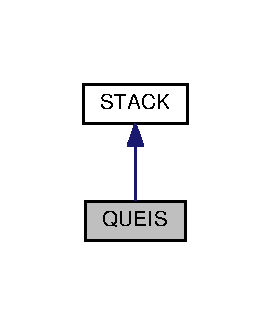
\includegraphics[width=130pt]{classQUEIS__coll__graph}
\end{center}
\end{figure}
\subsection*{Public 成员函数}
\begin{DoxyCompactItemize}
\item 
{\bfseries Q\+U\+E\+IS} (int m)\hypertarget{classQUEIS_a8eb66c1ff47e0f0aca03c563ac6e6dce}{}\label{classQUEIS_a8eb66c1ff47e0f0aca03c563ac6e6dce}

\item 
{\bfseries Q\+U\+E\+IS} (const \hyperlink{classQUEIS}{Q\+U\+E\+IS} \&q)\hypertarget{classQUEIS_ad9d0fe5e4b37f19883c5463173fd8ce6}{}\label{classQUEIS_ad9d0fe5e4b37f19883c5463173fd8ce6}

\item 
virtual {\bfseries operator int} (void) const \hypertarget{classQUEIS_a0cd5f9b0a81ad316af771078ea723873}{}\label{classQUEIS_a0cd5f9b0a81ad316af771078ea723873}

\item 
virtual \hyperlink{classQUEIS}{Q\+U\+E\+IS} \& {\bfseries operator$<$$<$} (int e)\hypertarget{classQUEIS_a6f9891ed65fb0e1127c31d1d9f2e85ee}{}\label{classQUEIS_a6f9891ed65fb0e1127c31d1d9f2e85ee}

\item 
virtual \hyperlink{classQUEIS}{Q\+U\+E\+IS} \& {\bfseries operator$>$$>$} (int \&e)\hypertarget{classQUEIS_acbf52122b69ca035a107cca9f4b73ab2}{}\label{classQUEIS_acbf52122b69ca035a107cca9f4b73ab2}

\item 
virtual \hyperlink{classQUEIS}{Q\+U\+E\+IS} \& {\bfseries operator=} (const \hyperlink{classQUEIS}{Q\+U\+E\+IS} \&q)\hypertarget{classQUEIS_a9b44dfb89316be0158361b642b7d558a}{}\label{classQUEIS_a9b44dfb89316be0158361b642b7d558a}

\item 
virtual void {\bfseries print} (void) const \hypertarget{classQUEIS_a447f31b50d9bea91fc5fc7c7aaffd68a}{}\label{classQUEIS_a447f31b50d9bea91fc5fc7c7aaffd68a}

\end{DoxyCompactItemize}


\subsection{详细描述}


在文件 queis.\+h 第 13 行定义.



该类的文档由以下文件生成\+:\begin{DoxyCompactItemize}
\item 
src/\hyperlink{queis_8h}{queis.\+h}\end{DoxyCompactItemize}

\hypertarget{classSTACK}{}\section{S\+T\+A\+C\+K类 参考}
\label{classSTACK}\index{S\+T\+A\+CK@{S\+T\+A\+CK}}


类 S\+T\+A\+CK 继承关系图\+:
\nopagebreak
\begin{figure}[H]
\begin{center}
\leavevmode
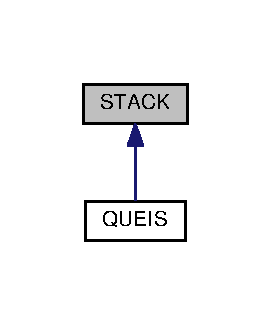
\includegraphics[width=130pt]{classSTACK__inherit__graph}
\end{center}
\end{figure}
\subsection*{Public 成员函数}
\begin{DoxyCompactItemize}
\item 
{\bfseries S\+T\+A\+CK} (int m)\hypertarget{classSTACK_a05bc9d50ad557a3674c526a89e86e448}{}\label{classSTACK_a05bc9d50ad557a3674c526a89e86e448}

\item 
{\bfseries S\+T\+A\+CK} (const \hyperlink{classSTACK}{S\+T\+A\+CK} \&s)\hypertarget{classSTACK_a3378f08d7a0a6eda56e19cec7259e188}{}\label{classSTACK_a3378f08d7a0a6eda56e19cec7259e188}

\item 
virtual int {\bfseries size} (void) const \hypertarget{classSTACK_a2c64a2e35765b1120870e5bd768a6094}{}\label{classSTACK_a2c64a2e35765b1120870e5bd768a6094}

\item 
virtual {\bfseries operator int} (void) const \hypertarget{classSTACK_aefb6f31671a86cedb35642f718999655}{}\label{classSTACK_aefb6f31671a86cedb35642f718999655}

\item 
virtual int {\bfseries operator\mbox{[}$\,$\mbox{]}} (int x) const \hypertarget{classSTACK_af623ee48118d6b41b13e37d8d90d76ac}{}\label{classSTACK_af623ee48118d6b41b13e37d8d90d76ac}

\item 
virtual \hyperlink{classSTACK}{S\+T\+A\+CK} \& {\bfseries operator$<$$<$} (int e)\hypertarget{classSTACK_ae0163e70963b3dc5b585ebddfa145542}{}\label{classSTACK_ae0163e70963b3dc5b585ebddfa145542}

\item 
virtual \hyperlink{classSTACK}{S\+T\+A\+CK} \& {\bfseries operator$>$$>$} (int \&e)\hypertarget{classSTACK_a8581b5dd2195110a1baa0bc39b222db7}{}\label{classSTACK_a8581b5dd2195110a1baa0bc39b222db7}

\item 
virtual \hyperlink{classSTACK}{S\+T\+A\+CK} \& {\bfseries operator=} (const \hyperlink{classSTACK}{S\+T\+A\+CK} \&s)\hypertarget{classSTACK_af05d024de2a827a1812b2860bc86b65a}{}\label{classSTACK_af05d024de2a827a1812b2860bc86b65a}

\item 
virtual void {\bfseries print} (void) const \hypertarget{classSTACK_a7fbad0471b86e1572c19c91c11389e5f}{}\label{classSTACK_a7fbad0471b86e1572c19c91c11389e5f}

\end{DoxyCompactItemize}


\subsection{详细描述}


在文件 stack.\+h 第 13 行定义.



该类的文档由以下文件生成\+:\begin{DoxyCompactItemize}
\item 
src/\hyperlink{stack_8h}{stack.\+h}\end{DoxyCompactItemize}

\chapter{文件说明}
\hypertarget{oostk_8h}{}\section{src/oostk.h 文件参考}
\label{oostk_8h}\index{src/oostk.\+h@{src/oostk.\+h}}


header file for object-\/oriented stack  


\subsection*{类}
\begin{DoxyCompactItemize}
\item 
class \hyperlink{classOOSTK}{O\+O\+S\+TK}
\end{DoxyCompactItemize}


\subsection{详细描述}
header file for object-\/oriented stack 

\begin{DoxyAuthor}{作者}
sabertazimi, \href{mailto:sabertazimi@gmail.com}{\tt sabertazimi@gmail.\+com} 
\end{DoxyAuthor}
\begin{DoxyVersion}{版本}
1.\+0 
\end{DoxyVersion}
\begin{DoxyDate}{日期}
2016-\/09-\/30 
\end{DoxyDate}

\hypertarget{postk_8h}{}\section{src/postk.h 文件参考}
\label{postk_8h}\index{src/postk.\+h@{src/postk.\+h}}


header file for process-\/oriented stack  


\subsection*{类}
\begin{DoxyCompactItemize}
\item 
struct \hyperlink{structPOSTK}{P\+O\+S\+TK}
\end{DoxyCompactItemize}
\subsection*{函数}
\begin{DoxyCompactItemize}
\item 
void \hyperlink{postk_8h_a404a25d222d39742da59078e22fc3580}{init\+P\+O\+S\+TK} (\hyperlink{structPOSTK}{P\+O\+S\+TK} $\ast$const p, int m)
\begin{DoxyCompactList}\small\item\em initiate stack \end{DoxyCompactList}\item 
void \hyperlink{postk_8h_af1665b700d0cc8dce05f76d4dbdc537b}{init\+P\+O\+S\+TK} (\hyperlink{structPOSTK}{P\+O\+S\+TK} $\ast$const p, const \hyperlink{structPOSTK}{P\+O\+S\+TK} \&s)
\begin{DoxyCompactList}\small\item\em initiate stack (with copy) \end{DoxyCompactList}\item 
int \hyperlink{postk_8h_adeefb25cecd4f0f14ce696ea9682a92f}{size} (const \hyperlink{structPOSTK}{P\+O\+S\+TK} $\ast$const p)
\begin{DoxyCompactList}\small\item\em get capacity of stack \end{DoxyCompactList}\item 
int \hyperlink{postk_8h_a4f550fadb28c4f42f2e1b60a5888cdf9}{how\+Many} (const \hyperlink{structPOSTK}{P\+O\+S\+TK} $\ast$const p)
\begin{DoxyCompactList}\small\item\em get number of elements in stack \end{DoxyCompactList}\item 
int \hyperlink{postk_8h_afe57536dc8ba014ab6e7fa599eab69b2}{getelem} (const \hyperlink{structPOSTK}{P\+O\+S\+TK} $\ast$const p, int x)
\begin{DoxyCompactList}\small\item\em get target element with index x \end{DoxyCompactList}\item 
\hyperlink{structPOSTK}{P\+O\+S\+TK} $\ast$const \hyperlink{postk_8h_a851f4ffbd1543203140109d131e519c3}{push} (\hyperlink{structPOSTK}{P\+O\+S\+TK} $\ast$const p, int e)
\begin{DoxyCompactList}\small\item\em push a new element into stack \end{DoxyCompactList}\item 
\hyperlink{structPOSTK}{P\+O\+S\+TK} $\ast$const \hyperlink{postk_8h_a27a5bf5d58c0d27cabb02ea54d336086}{pop} (\hyperlink{structPOSTK}{P\+O\+S\+TK} $\ast$const p, int \&e)
\begin{DoxyCompactList}\small\item\em pop a element from stack \end{DoxyCompactList}\item 
\hyperlink{structPOSTK}{P\+O\+S\+TK} $\ast$const \hyperlink{postk_8h_a19a767cf1ee7dfbba6a40a8d029c26f3}{assign} (\hyperlink{structPOSTK}{P\+O\+S\+TK} $\ast$const p, const \hyperlink{structPOSTK}{P\+O\+S\+TK} \&s)
\begin{DoxyCompactList}\small\item\em assign stack of p with stack of s \end{DoxyCompactList}\item 
void \hyperlink{postk_8h_af82cdfbc18d1fa4f3c8b2ce2cd0347f1}{print} (const \hyperlink{structPOSTK}{P\+O\+S\+TK} $\ast$const p)
\begin{DoxyCompactList}\small\item\em print all elements in stack \end{DoxyCompactList}\item 
void \hyperlink{postk_8h_ac6285f066faaaac13d297187eb102123}{destroy\+P\+O\+S\+TK} (\hyperlink{structPOSTK}{P\+O\+S\+TK} $\ast$const p)
\begin{DoxyCompactList}\small\item\em destroy stack \end{DoxyCompactList}\end{DoxyCompactItemize}


\subsection{详细描述}
header file for process-\/oriented stack 

\begin{DoxyAuthor}{作者}
sabertazimi,\href{mailto:sabertazimi@gmail.com}{\tt sabertazimi@gmail.\+com} 
\end{DoxyAuthor}
\begin{DoxyVersion}{版本}
1.\+0 
\end{DoxyVersion}
\begin{DoxyDate}{日期}
2016-\/09-\/29 
\end{DoxyDate}


\subsection{函数说明}
\index{postk.\+h@{postk.\+h}!assign@{assign}}
\index{assign@{assign}!postk.\+h@{postk.\+h}}
\subsubsection[{\texorpdfstring{assign(\+P\+O\+S\+T\+K $\ast$const p, const P\+O\+S\+T\+K \&s)}{assign(POSTK *const p, const POSTK &s)}}]{\setlength{\rightskip}{0pt plus 5cm}{\bf P\+O\+S\+TK}$\ast$ const assign (
\begin{DoxyParamCaption}
\item[{{\bf P\+O\+S\+TK} $\ast$const}]{p, }
\item[{const {\bf P\+O\+S\+TK} \&}]{s}
\end{DoxyParamCaption}
)}\hypertarget{postk_8h_a19a767cf1ee7dfbba6a40a8d029c26f3}{}\label{postk_8h_a19a767cf1ee7dfbba6a40a8d029c26f3}


assign stack of p with stack of s 


\begin{DoxyParams}{参数}
{\em p} & destination stack pointer \\
\hline
{\em s} & source stack pointer \\
\hline
\end{DoxyParams}
\begin{DoxyReturn}{返回}
stack pointer point to p 
\end{DoxyReturn}
\index{postk.\+h@{postk.\+h}!destroy\+P\+O\+S\+TK@{destroy\+P\+O\+S\+TK}}
\index{destroy\+P\+O\+S\+TK@{destroy\+P\+O\+S\+TK}!postk.\+h@{postk.\+h}}
\subsubsection[{\texorpdfstring{destroy\+P\+O\+S\+T\+K(\+P\+O\+S\+T\+K $\ast$const p)}{destroyPOSTK(POSTK *const p)}}]{\setlength{\rightskip}{0pt plus 5cm}void destroy\+P\+O\+S\+TK (
\begin{DoxyParamCaption}
\item[{{\bf P\+O\+S\+TK} $\ast$const}]{p}
\end{DoxyParamCaption}
)}\hypertarget{postk_8h_ac6285f066faaaac13d297187eb102123}{}\label{postk_8h_ac6285f066faaaac13d297187eb102123}


destroy stack 


\begin{DoxyParams}{参数}
{\em p} & stack pointer \\
\hline
\end{DoxyParams}
\begin{DoxyReturn}{返回}
void 
\end{DoxyReturn}
\index{postk.\+h@{postk.\+h}!getelem@{getelem}}
\index{getelem@{getelem}!postk.\+h@{postk.\+h}}
\subsubsection[{\texorpdfstring{getelem(const P\+O\+S\+T\+K $\ast$const p, int x)}{getelem(const POSTK *const p, int x)}}]{\setlength{\rightskip}{0pt plus 5cm}int getelem (
\begin{DoxyParamCaption}
\item[{const {\bf P\+O\+S\+TK} $\ast$const}]{p, }
\item[{int}]{x}
\end{DoxyParamCaption}
)}\hypertarget{postk_8h_afe57536dc8ba014ab6e7fa599eab69b2}{}\label{postk_8h_afe57536dc8ba014ab6e7fa599eab69b2}


get target element with index x 


\begin{DoxyParams}{参数}
{\em p} & stack pointer \\
\hline
{\em x} & index of target element \\
\hline
\end{DoxyParams}
\begin{DoxyReturn}{返回}
tartget element with index x 
\end{DoxyReturn}
\index{postk.\+h@{postk.\+h}!how\+Many@{how\+Many}}
\index{how\+Many@{how\+Many}!postk.\+h@{postk.\+h}}
\subsubsection[{\texorpdfstring{how\+Many(const P\+O\+S\+T\+K $\ast$const p)}{howMany(const POSTK *const p)}}]{\setlength{\rightskip}{0pt plus 5cm}int how\+Many (
\begin{DoxyParamCaption}
\item[{const {\bf P\+O\+S\+TK} $\ast$const}]{p}
\end{DoxyParamCaption}
)}\hypertarget{postk_8h_a4f550fadb28c4f42f2e1b60a5888cdf9}{}\label{postk_8h_a4f550fadb28c4f42f2e1b60a5888cdf9}


get number of elements in stack 


\begin{DoxyParams}{参数}
{\em p} & stack pointer \\
\hline
\end{DoxyParams}
\begin{DoxyReturn}{返回}
number of elements in stack 
\end{DoxyReturn}
\index{postk.\+h@{postk.\+h}!init\+P\+O\+S\+TK@{init\+P\+O\+S\+TK}}
\index{init\+P\+O\+S\+TK@{init\+P\+O\+S\+TK}!postk.\+h@{postk.\+h}}
\subsubsection[{\texorpdfstring{init\+P\+O\+S\+T\+K(\+P\+O\+S\+T\+K $\ast$const p, int m)}{initPOSTK(POSTK *const p, int m)}}]{\setlength{\rightskip}{0pt plus 5cm}void init\+P\+O\+S\+TK (
\begin{DoxyParamCaption}
\item[{{\bf P\+O\+S\+TK} $\ast$const}]{p, }
\item[{int}]{m}
\end{DoxyParamCaption}
)}\hypertarget{postk_8h_a404a25d222d39742da59078e22fc3580}{}\label{postk_8h_a404a25d222d39742da59078e22fc3580}


initiate stack 


\begin{DoxyParams}{参数}
{\em p} & stack pointer \\
\hline
{\em m} & stack capacity \\
\hline
\end{DoxyParams}
\begin{DoxyReturn}{返回}
void 
\end{DoxyReturn}
\index{postk.\+h@{postk.\+h}!init\+P\+O\+S\+TK@{init\+P\+O\+S\+TK}}
\index{init\+P\+O\+S\+TK@{init\+P\+O\+S\+TK}!postk.\+h@{postk.\+h}}
\subsubsection[{\texorpdfstring{init\+P\+O\+S\+T\+K(\+P\+O\+S\+T\+K $\ast$const p, const P\+O\+S\+T\+K \&s)}{initPOSTK(POSTK *const p, const POSTK &s)}}]{\setlength{\rightskip}{0pt plus 5cm}void init\+P\+O\+S\+TK (
\begin{DoxyParamCaption}
\item[{{\bf P\+O\+S\+TK} $\ast$const}]{p, }
\item[{const {\bf P\+O\+S\+TK} \&}]{s}
\end{DoxyParamCaption}
)}\hypertarget{postk_8h_af1665b700d0cc8dce05f76d4dbdc537b}{}\label{postk_8h_af1665b700d0cc8dce05f76d4dbdc537b}


initiate stack (with copy) 


\begin{DoxyParams}{参数}
{\em p} & destination stack pointer \\
\hline
{\em s} & source stack pointer \\
\hline
\end{DoxyParams}
\begin{DoxyReturn}{返回}
void 
\end{DoxyReturn}
\index{postk.\+h@{postk.\+h}!pop@{pop}}
\index{pop@{pop}!postk.\+h@{postk.\+h}}
\subsubsection[{\texorpdfstring{pop(\+P\+O\+S\+T\+K $\ast$const p, int \&e)}{pop(POSTK *const p, int &e)}}]{\setlength{\rightskip}{0pt plus 5cm}{\bf P\+O\+S\+TK}$\ast$ const pop (
\begin{DoxyParamCaption}
\item[{{\bf P\+O\+S\+TK} $\ast$const}]{p, }
\item[{int \&}]{e}
\end{DoxyParamCaption}
)}\hypertarget{postk_8h_a27a5bf5d58c0d27cabb02ea54d336086}{}\label{postk_8h_a27a5bf5d58c0d27cabb02ea54d336086}


pop a element from stack 


\begin{DoxyParams}{参数}
{\em p} & stack pointer \\
\hline
{\em e} & hold value of element poped \\
\hline
\end{DoxyParams}
\begin{DoxyReturn}{返回}
stack pointer point to p 
\end{DoxyReturn}
\index{postk.\+h@{postk.\+h}!print@{print}}
\index{print@{print}!postk.\+h@{postk.\+h}}
\subsubsection[{\texorpdfstring{print(const P\+O\+S\+T\+K $\ast$const p)}{print(const POSTK *const p)}}]{\setlength{\rightskip}{0pt plus 5cm}void print (
\begin{DoxyParamCaption}
\item[{const {\bf P\+O\+S\+TK} $\ast$const}]{p}
\end{DoxyParamCaption}
)}\hypertarget{postk_8h_af82cdfbc18d1fa4f3c8b2ce2cd0347f1}{}\label{postk_8h_af82cdfbc18d1fa4f3c8b2ce2cd0347f1}


print all elements in stack 


\begin{DoxyParams}{参数}
{\em p} & stack pointer \\
\hline
\end{DoxyParams}
\begin{DoxyReturn}{返回}
void 
\end{DoxyReturn}
\index{postk.\+h@{postk.\+h}!push@{push}}
\index{push@{push}!postk.\+h@{postk.\+h}}
\subsubsection[{\texorpdfstring{push(\+P\+O\+S\+T\+K $\ast$const p, int e)}{push(POSTK *const p, int e)}}]{\setlength{\rightskip}{0pt plus 5cm}{\bf P\+O\+S\+TK}$\ast$ const push (
\begin{DoxyParamCaption}
\item[{{\bf P\+O\+S\+TK} $\ast$const}]{p, }
\item[{int}]{e}
\end{DoxyParamCaption}
)}\hypertarget{postk_8h_a851f4ffbd1543203140109d131e519c3}{}\label{postk_8h_a851f4ffbd1543203140109d131e519c3}


push a new element into stack 


\begin{DoxyParams}{参数}
{\em p} & stack pointer \\
\hline
{\em e} & new element to push \\
\hline
\end{DoxyParams}
\begin{DoxyReturn}{返回}
stack pointer point to p 
\end{DoxyReturn}
\index{postk.\+h@{postk.\+h}!size@{size}}
\index{size@{size}!postk.\+h@{postk.\+h}}
\subsubsection[{\texorpdfstring{size(const P\+O\+S\+T\+K $\ast$const p)}{size(const POSTK *const p)}}]{\setlength{\rightskip}{0pt plus 5cm}int size (
\begin{DoxyParamCaption}
\item[{const {\bf P\+O\+S\+TK} $\ast$const}]{p}
\end{DoxyParamCaption}
)}\hypertarget{postk_8h_adeefb25cecd4f0f14ce696ea9682a92f}{}\label{postk_8h_adeefb25cecd4f0f14ce696ea9682a92f}


get capacity of stack 


\begin{DoxyParams}{参数}
{\em p} & stack pointer \\
\hline
\end{DoxyParams}
\begin{DoxyReturn}{返回}
capacity of stack 
\end{DoxyReturn}

\hypertarget{que2s_8h}{}\section{src/que2s.h 文件参考}
\label{que2s_8h}\index{src/que2s.\+h@{src/que2s.\+h}}


header file for queue consisting of 2 stack  


\subsection*{类}
\begin{DoxyCompactItemize}
\item 
class \hyperlink{classQUE2S}{Q\+U\+E2S}
\end{DoxyCompactItemize}


\subsection{详细描述}
header file for queue consisting of 2 stack 

\begin{DoxyAuthor}{作者}
sabertazimi, \href{mailto:sabertazimi@gmail.com}{\tt sabertazimi@gmail.\+com} 
\end{DoxyAuthor}
\begin{DoxyVersion}{版本}
1.\+0 
\end{DoxyVersion}
\begin{DoxyDate}{日期}
2016-\/09-\/30 
\end{DoxyDate}

\hypertarget{queis_8h}{}\section{src/queis.h 文件参考}
\label{queis_8h}\index{src/queis.\+h@{src/queis.\+h}}


header file for queue inheriting from stack  


\subsection*{类}
\begin{DoxyCompactItemize}
\item 
class \hyperlink{classQUEIS}{Q\+U\+E\+IS}
\end{DoxyCompactItemize}


\subsection{详细描述}
header file for queue inheriting from stack 

\begin{DoxyAuthor}{作者}
sabertazimi, \href{mailto:sabertazimi@gmail.com}{\tt sabertazimi@gmail.\+com} 
\end{DoxyAuthor}
\begin{DoxyVersion}{版本}
1.\+0 
\end{DoxyVersion}
\begin{DoxyDate}{日期}
2016-\/09-\/30 
\end{DoxyDate}

\hypertarget{stack_8h}{}\section{src/stack.h 文件参考}
\label{stack_8h}\index{src/stack.\+h@{src/stack.\+h}}


header file for operator overload object-\/oriented stack  


\subsection*{类}
\begin{DoxyCompactItemize}
\item 
class \hyperlink{classSTACK}{S\+T\+A\+CK}
\end{DoxyCompactItemize}


\subsection{详细描述}
header file for operator overload object-\/oriented stack 

\begin{DoxyAuthor}{作者}
sabertazimi, \href{mailto:sabertazimi@gmail.com}{\tt sabertazimi@gmail.\+com} 
\end{DoxyAuthor}
\begin{DoxyVersion}{版本}
1.\+0 
\end{DoxyVersion}
\begin{DoxyDate}{日期}
2016-\/09-\/30 
\end{DoxyDate}

%--- End generated contents ---

% Index
\backmatter
\newpage
\phantomsection
\clearemptydoublepage
\addcontentsline{toc}{chapter}{索引}
\printindex

\end{document}
